\subsection{CSS 3}

\citeonline{silva_css_3}, afirma que a principal função do \textit{Cascading Style Sheet} - CSS\footnotemark[25] - é definir como os componentes anteriormente estruturados nos documentos \textit{web}, por meio do HTML devem ser apresentados ao usuário.

\footnotetext[25]{CSS: \textit{Cascading Style Sheet} - Documentos que definem estilos aos componentes da página \textit{web}.}

Para \citeonline{w3c_css_definition}, o CSS é ''\textit{a simple mechanism for adding style (e.g., fonts, colors, spacing) to Web documents}\footnotemark[26]''.

\footnotetext[26]{O CSS é um simples mecanismo para adicionar estilo, como: fontes, cores, espaços para os documentos \textit{Web}.}

Tim Berners-Lee, inicialmente escrevia as estilizações de seus documentos \textit{web}, mesmo que de forma simples e limitada, nos próprios documentos HTML. Isto se deve ao fato de que, ele acreditava que tal função deveria ser realizada pelos navegadores. Entretanto, em 1994 a primeira proposta de criação do CSS surgiu e em 1996, a primeira versão do CSS denominada CSS 1 foi lançada como recomendação do W3C \cite{silva_css_3}.

De acordo com \citeonline{silva_css_3}, Atualmente o CSS possui 4 versões: A CSS 1, a 2, a 2.1 e atualmente a 3.


Há 3 formas de incorporar o CSS em seu documento web segundo \cite{silva_css_3}, são elas: 

\begin{itemize}
	\item \textbf{\textit{Inline}:} É possível aplicar o estilo diretamente ao componente desejado, por meio do uso da propriedade \texttt{style} do componente HTML. Como é apresentado na figura 10;
	
	\newpage
	\begin{figure}[h!]
		\centerline{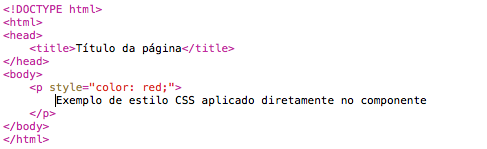
\includegraphics[scale=0.8]{./imagens/example_css_inline.png}}
		\caption[Exemplo de inclusão do estilo CSS inline]
		{Exemplo de inclusão do estilo CSS inline. \textbf{Fonte:} Elaborado pelos autores.}
		\label{fig:exemplo1}
	\end{figure}
	
	\item \textbf{Incorporado:} Outra forma, é escrever todo CSS referente ao  documento \textit{web} dentro da \textit{tag} \texttt{style} do documento HTML. Para tanto, esta \textit{tag} deve ser inserida entre o início e o fim da \textit{tag} \texttt{head} do documento. Como é apresentado na figura 11;
	
	\begin{figure}[h!]
		\centerline{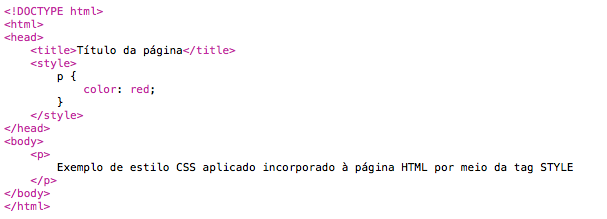
\includegraphics[scale=0.8]{./imagens/example_css_incorpored.png}}
		\caption[Exemplo de inclusão do estilo CSS incorporado à página HTML]
		{Exemplo de inclusão do estilo CSS incorporado à página HTML. \textbf{Fonte:} Elaborado pelos autores.}
		\label{fig:exemplo1}
	\end{figure}
	 
	\item \textbf{Externo:} A última forma, é criar um arquivo externo com extensão \texttt{.css} e definir todas as regras de estilização do documento \textit{web} neste arquivo. Desta forma, para vincular tal arquivo à um documento HTML específico será necessário utilizar a \textit{tag} \texttt{link} entre o início e o fim da \textit{tag} \texttt{head} do documento. Como é apresentado na figura 12;
	
	\newpage
	\begin{figure}[h!]
		\centerline{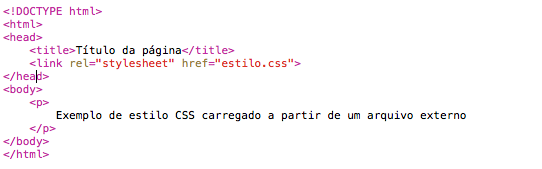
\includegraphics[scale=0.8]{./imagens/example_external_css.png}}
		\caption[Exemplo de inclusão do estilo CSS a partir de um arquivo externo]
		{Exemplo de inclusão do estilo CSS a partir de um arquivo externo. \textbf{Fonte:} Elaborado pelos autores.}
		\label{fig:exemplo1}
	\end{figure}
	
\end{itemize}

O CSS 3 será utilizado neste projeto, pois, ele permite definir estilos aos componentes das páginas \textit{web} e possui recursos que não são existem em suas versões anteriores, o que nos permite desenvolver páginas mais atrativas com menos recursos.